\chapter{System Overview}
\label{sec:system_overview}

This chapter provides a comprehensive description of the personalized-ai-storybook system architecture, design patterns, and technical implementation for the FYP-2 phase. The system integrates six major new modules (TTS, STT, styled PDF, evaluation, and UI enhancements) into the existing multi-agent pipeline.

\section{Architectural Design}

personalized-ai-storybook employs a layered architecture pattern to achieve modularity, maintainability, and clarity of responsibility. The architecture consists of six distinct layers, each with well-defined responsibilities and clear interfaces for inter-layer communication.

\subsection{Architecture Layers}

\textbf{1. Presentation Layer (Frontend)} \\
The topmost layer handles all user interactions and visual presentation. It comprises the Next.js-based UI with TypeScript, including:
\begin{itemize}
    \item Landing page with mode selection (Simple vs.\ Personalized)
    \item Multi-modal input interface: text prompt field, voice input button (STT), and file upload (personalized photo)
    \item Open-book story display: illustration left page, story text right page, page-flip navigation
    \item Per-page audio controls (play/pause, voice selector) for TTS playback
    \item Character Chatbot and Idea Workshop panels
    \item Theme toggle (light/dark mode) and customization dropdowns (genre, style, length)
\end{itemize}

\textbf{2. Application Layer (Backend API)} \\
FastAPI (main.py) acts as the entry point for all backend operations:
\begin{itemize}
    \item \texttt{POST /api/generate} — Story generation (simple or personalized)
    \item \texttt{POST /api/tts} — Audio narration generation/retrieval
    \item \texttt{POST /api/stt} — Speech-to-text transcription
    \item \texttt{POST /api/chat} — Character chatbot interaction
    \item \texttt{POST /api/workshop/session} and \texttt{/message} — Idea workshop
    \item \texttt{GET /api/stories} — User story history
    \item \texttt{GET /device} — Hardware detection (GPU/CPU)
\end{itemize}

\textbf{3. Business Logic Layer (Multi-Agent System)} \\
This layer contains the core domain logic and specialized agent implementations:
\begin{itemize}
    \item \textbf{PromptAgent} — Input validation, enhancement, classification
    \item \textbf{DirectorAgent} — Orchestrates the Writer → Reviewer → Editor pipeline
    \item \textbf{WriterAgent} — Story generation via Ollama LLM
    \item \textbf{ReviewerAgent} — Quality assurance and age-appropriateness
    \item \textbf{EditorAgent} — Final polish and PDF export (ReportLab open-book layout)
    \item \textbf{ImageAgent} — Standard Stable Diffusion image generation
    \item \textbf{PersonalizedImageAgent} — IP-Adapter FaceID Plus v2 via WebUI API
    \item \textbf{ChatbotAgent} — Story-context-aware character conversations
    \item \textbf{IdeaWorkshopAgent} — LangChain-based multi-turn story ideation
    \item \textbf{EvaluationAgent} — Asynchronous quality metrics computation
\end{itemize}

\textbf{4. AI/ML Layer (Model Inference)} \\
The most computationally intensive layer:
\begin{itemize}
    \item \textbf{Ollama} — Local LLM inference (llama3.1:8b-instruct-q4\_K\_M, mistral-nemo:12b for workshop)
    \item \textbf{Stable Diffusion WebUI} — Image generation with IP-Adapter; txt2img + img2img pipeline
    \item \textbf{Piper TTS} — Offline ONNX text-to-speech synthesis
    \item \textbf{OpenAI Whisper} — Offline speech-to-text transcription
    \item \textbf{CLIP} (ViT-B/32) — Image-text alignment and visual consistency evaluation
    \item \textbf{Sentence Transformers} — Text coherence evaluation
    \item \textbf{InsightFace} — Character face consistency evaluation (personalized mode)
    \item \textbf{PyTorch} — Tensor operations and device management (CUDA/CPU)
\end{itemize}

\textbf{5. Data Layer (Hybrid Storage)} \\
\begin{itemize}
    \item \textbf{PostgreSQL} (SQLAlchemy ORM) — Users, stories, chat sessions, workshop sessions and messages
    \item \textbf{File System} — \texttt{generated/images/}, \texttt{generated/audio/}, \texttt{generated/exports/}, \texttt{generated/evaluations/}, \texttt{generated/stories/}
\end{itemize}

\textbf{6. Infrastructure Layer} \\
\begin{itemize}
    \item OllamaManager — GPU memory management (pause/resume Ollama during image generation)
    \item ContentSafety — Blocked/warning keyword filtering for prompts and image descriptions
    \item EvaluationManager — Singleton evaluation orchestrator with lazy model loading
    \item TTSManager — Singleton Piper TTS with audio caching
    \item WhisperSTTManager — Singleton Whisper with ffmpeg-free WAV reader
\end{itemize}

\subsection{Key Design Patterns}

\textbf{Facade Pattern}: The \texttt{StoryAgent} class provides a simplified interface to the complex multi-agent pipeline orchestrated by the \texttt{DirectorAgent}. \\
\textbf{Pipeline Pattern}: Story generation follows a sequential pipeline — Prompt Agent → Writer Agent → Reviewer Agent → Editor Agent — where each agent transforms and passes data to the next stage. \\
\textbf{Singleton Pattern}: \texttt{TTSManager}, \texttt{WhisperSTTManager}, and \texttt{EvaluationManager} are all singletons, ensuring models are loaded once and reused across requests. \\
\textbf{Strategy Pattern}: The \texttt{generate\_images} flag and \texttt{use\_personalized\_images} flag act as strategy selectors, choosing between text-only, standard, or personalized image generation. \\
\textbf{Observer Pattern (Async)}: The \texttt{EvaluationAgent} is triggered asynchronously after story completion, observing the completed story without blocking the main response.


\section{Design Models}

This section presents detailed design models capturing the system's behavior, structure, and data flow.

\subsection{Use Case Diagram}

The use case diagram illustrates the primary interactions between two actor types --- the \textbf{Registered User} and the \textbf{System (Background)} --- and the eight core use cases of personalized-ai-storybook FYP-2.

\begin{figure}[H]
    \centering
    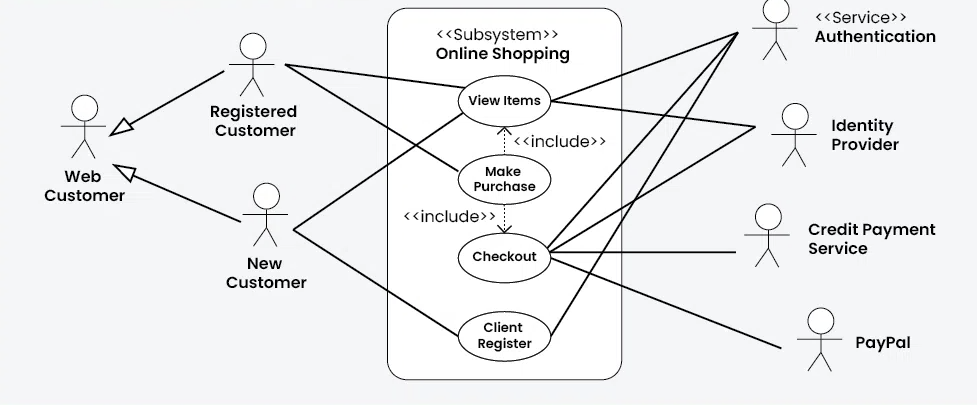
\includegraphics[width=\textwidth]{images/usecaseexample.png}
    \caption{Use Case Diagram -- personalized-ai-storybook FYP-2 (see diagram file: \texttt{diagrams/use\_case.puml})}
    \label{fig:usecase}
\end{figure}

\textbf{Actors and Use Cases:}
\begin{itemize}
    \item \textbf{Registered User}: Generate Story from Text (UC1), Generate Story from Voice (UC2), Listen to Narration (UC3), Generate Personalized Story (UC4), View Evaluation Metrics (UC5), Chat with Character (UC6), Idea Workshop (UC7), Export to PDF (UC8).
    \item \textbf{System (Background)}: Run Evaluation Agent (triggered automatically after generation).
\end{itemize}

\subsection{Activity Diagram}

The activity diagram illustrates the complete story generation workflow from user input to final output, covering both Simple and Personalized modes.

\textbf{Key Activities}:
\begin{enumerate}
    \item User selects mode (Simple / Personalized) and provides input (text or voice).
    \item [STT path] Audio is transcribed by Whisper; text is returned.
    \item Prompt Agent validates and enhances prompt; content safety check.
    \item Director Agent orchestrates: Writer → Reviewer → Editor.
    \item [Personalized path] IP-Adapter photo is processed; Ollama paused for GPU.
    \item Image Agent generates scene illustrations (txt2img → img2img).
    \item Editor Agent exports styled PDF (leather cover, notebook pages).
    \item Evaluation Agent runs asynchronously; results stored.
    \item Story displayed in open-book UI with TTS controls.
\end{enumerate}

\subsection{Data Flow Diagram}

The DFD models the data flow through the personalized-ai-storybook system across three levels.

\subsubsection{Context Diagram (DFD Level 0)}

The context diagram shows the system boundary and external entities:

\begin{itemize}
    \item \textbf{External Entities}: User (provides prompts, voice audio, reference photos; receives stories, audio, PDFs), Ollama Server (LLM inference), Stable Diffusion WebUI (image generation), PostgreSQL Database (data persistence).
    \item \textbf{Central Process}: personalized-ai-storybook System (receives inputs, produces storybook outputs).
    \item \textbf{Data Flows}: User Prompt → System; Voice Audio → System; Reference Photo → System; Story JSON ← System; Audio WAV ← System; PDF ← System.
\end{itemize}

\begin{figure}[H]
    \centering
    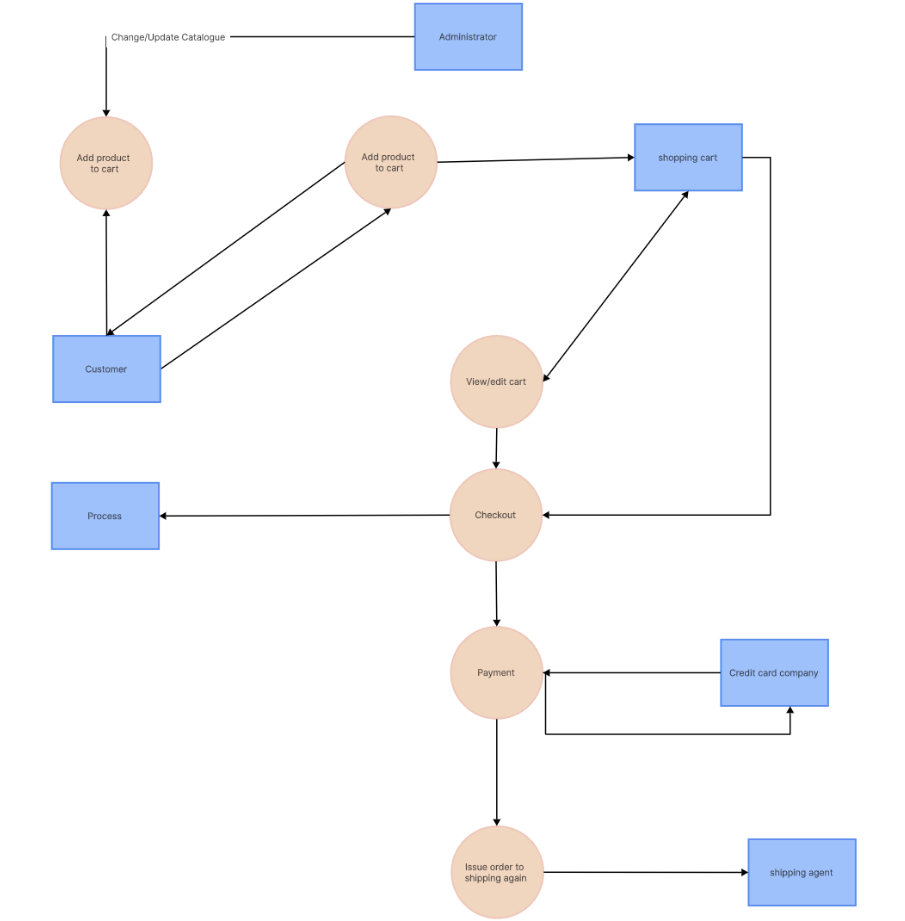
\includegraphics[width=0.85\textwidth]{images/dfd.png}
    \caption{Context Diagram (DFD Level 0) -- personalized-ai-storybook (see: \texttt{diagrams/dfd\_context.puml})}
    \label{fig:dfd_context}
\end{figure}

\subsubsection{Level 1 DFD}

The Level 1 DFD decomposes the system into six main processes:

\begin{enumerate}
    \item \textbf{1.0 Process User Input} — Receives text/voice, validates, converts STT; outputs: enhanced prompt.
    \item \textbf{2.0 Generate Story Text} — Multi-agent pipeline (Writer/Reviewer/Editor); reads/writes STORIES store; outputs: story JSON.
    \item \textbf{3.0 Generate Illustrations} — Receives scene descriptions; writes IMAGES store; outputs: image paths.
    \item \textbf{4.0 Synthesize Audio} — Receives scene text; reads/writes AUDIO store; outputs: WAV paths.
    \item \textbf{5.0 Export PDF} — Receives story+images; writes EXPORTS store; outputs: PDF path.
    \item \textbf{6.0 Evaluate Quality} — Receives story+images; writes EVALUATIONS store; outputs: metrics JSON.
\end{enumerate}

\subsubsection{Level 2 DFD -- Story Generation (Process 2.0)}

Process 2.0 expands into:
\begin{itemize}
    \item \textbf{2.1 Validate \& Enhance Prompt} (Prompt Agent): receives raw prompt → outputs enhanced prompt.
    \item \textbf{2.2 Generate Story Draft} (Writer Agent): calls Ollama; retries on JSON failure; outputs story draft.
    \item \textbf{2.3 Review Story} (Reviewer Agent): checks coherence/age-appropriateness; outputs reviewed story.
    \item \textbf{2.4 Edit \& Finalize} (Editor Agent): polishes text; saves to STORIES store; triggers PDF export.
\end{itemize}

\subsection{Class Diagram}

The class diagram illustrates the object-oriented structure, showing the key agent classes, their attributes, methods, and relationships. See the diagram files for the full PlantUML source (\texttt{diagrams/class\_diagram.puml}).

\textbf{Key Classes and Relationships}:
\begin{itemize}
    \item \textbf{DirectorAgent} (orchestrator) → aggregates WriterAgent, ReviewerAgent, EditorAgent, ImageAgent.
    \item \textbf{StoryAgent} (facade) → delegates to DirectorAgent.
    \item \textbf{PersonalizedImageAgent} (extends ImageAgent) → uses WebUI API with IP-Adapter.
    \item \textbf{ChatbotAgent} — depends on Story (context); associated with ChatConversation.
    \item \textbf{IdeaWorkshopAgent} — aggregates WorkshopSession and WorkshopMessage.
    \item \textbf{TTSManager} (singleton) — generates/caches WAV files.
    \item \textbf{WhisperSTTManager} (singleton) — transcribes WAV audio.
    \item \textbf{EvaluationManager} (singleton) — orchestrates all evaluation metrics.

\end{itemize}

\subsection{Sequence Diagram: TTS Audio Narration}

This sequence diagram illustrates the Text-to-Speech audio generation flow:
\begin{enumerate}
    \item User clicks ``Play'' on story page; frontend sends \texttt{POST /api/tts} with \{story\_id, scene\_number, voice\}.
    \item FastAPI routes request to \texttt{TTSManager.generate\_audio()}.
    \item TTSManager checks audio cache; if exists, returns cached relative path.
    \item If not cached: writes scene text to temp file; invokes Piper TTS subprocess via PowerShell.
    \item WAV file saved to \texttt{generated/audio/}; path returned to frontend.
    \item Frontend loads audio from static file route and plays through browser audio element.
\end{enumerate}

\subsection{Sequence Diagram: STT Voice Input}

\begin{enumerate}
    \item User clicks voice input button; browser records audio and sends WAV to \texttt{POST /api/stt}.
    \item FastAPI saves WAV to temp file; calls \texttt{WhisperSTTManager.transcribe\_audio()}.
    \item STT manager reads WAV using built-in \texttt{wave} module (no ffmpeg); converts to float32 numpy array.
    \item Audio resampled from original rate to 16kHz using numpy linear interpolation.
    \item Whisper model transcribes audio; returns \{text, language\}.
    \item FastAPI returns transcribed text to frontend; pre-filled in prompt field.
\end{enumerate}

\subsection{State Transition Diagram}

The state diagram models the lifecycle of a Story object within the system:

\textbf{States}: IDLE → PROMPT\_RECEIVED → VALIDATING → GENERATING\_TEXT → REVIEWING → EDITING → GENERATING\_IMAGES (optional) → EXPORTING\_PDF → EVALUATING (background) → COMPLETED → NARRATING (on user demand) \\
\textbf{Key Transitions}:
\begin{itemize}
    \item IDLE → PROMPT\_RECEIVED: User submits prompt (text or via STT).
    \item GENERATING\_IMAGES → EXPORTING\_PDF: Image generation completes (or times out).
    \item COMPLETED → NARRATING: User clicks play on any scene page.
    \item Any state → ERROR: On unrecoverable exception; system logs and returns error response.
\end{itemize}


\section{Data Design}

The system uses a hybrid data storage approach: structured PostgreSQL for user/session data and file-based storage for generated content.

\subsection{Database Schema}

The PostgreSQL database consists of 7 tables managed via SQLAlchemy ORM:

\begin{itemize}
    \item \textbf{Users}: id, username, email, hashed\_password, created\_at.
    \item \textbf{Stories}: id, user\_id (FK), title, story\_json, pdf\_path, mode, created\_at.
    \item \textbf{ChatConversations}: id, story\_id (FK), character\_name, created\_at.
    \item \textbf{ChatMessages}: id, conversation\_id (FK), role, content, timestamp.
    \item \textbf{WorkshopSessions}: id, user\_id (FK), mode, status, created\_at.
    \item \textbf{WorkshopMessages}: id, session\_id (FK), role, content, metadata, timestamp.
    \item \textbf{WorkshopStories}: id, session\_id (FK), story\_json, version, created\_at.
\end{itemize}

\subsection{File System Storage}

Generated content is organized in dedicated directories under \texttt{generated/}:
\begin{itemize}
    \item \texttt{images/} — PNG scene illustrations (timestamped filenames).
    \item \texttt{audio/} — WAV narration files (story\_\{id\}\_scene\_\{n\}\_\{voice\}.wav).
    \item \texttt{exports/} — Styled PDF storybooks.
    \item \texttt{evaluations/} — JSON quality metrics reports.
    \item \texttt{stories/} — Final JSON story objects.
    \item \texttt{drafts/}, \texttt{prompts/}, \texttt{reviews/}, \texttt{edits/} — Agent intermediate outputs.
\end{itemize}

\subsection{JSON Story Structure}

Stories are represented in a standardized JSON schema validated by Pydantic:
\begin{itemize}
    \item \texttt{title}: String story title.
    \item \texttt{setting}: String describing the story world.
    \item \texttt{characters}: Array of character names.
    \item \texttt{scenes}: Array of \{scene\_number, text, image\_description, image\_path, image\_url\}.
    \item \texttt{meta}: Optional metadata (genre, style, prompt\_type, enhanced\_prompt, mode).
    \item \texttt{mode}: ``simple'' | ``personalized''.
    \item \texttt{finalized}: Boolean; true after EditorAgent completes.
\end{itemize}


\section{Domain Model}

The domain model represents the core business entities and their relationships in personalized-ai-storybook FYP-2:

\begin{itemize}
    \item \textbf{User}: Authenticated platform user; creates Stories; participates in WorkshopSessions.
    \item \textbf{Story}: A complete generated storybook with title, setting, characters, scenes, metadata, mode, and optional audio paths.
    \item \textbf{Scene}: Individual page of a story with text, image description, image path, and audio path.
    \item \textbf{Agent (Abstract)}: Base for PromptAgent, WriterAgent, ReviewerAgent, EditorAgent, ImageAgent, PersonalizedImageAgent, ChatbotAgent, IdeaWorkshopAgent, EvaluationAgent.
    \item \textbf{TTSManager}: Generates and caches WAV narration per scene.
    \item \textbf{WhisperSTTManager}: Transcribes user voice input.
    \item \textbf{EvaluationReport}: Quality assessment result with per-metric scores and overall weighted score.
    \item \textbf{WorkshopSession}: Interactive story ideation session with conversation history.
    \item \textbf{ChatConversation}: Character chatbot session linked to a specific Story.
\end{itemize}
